\section{Quality Requirements}

\subsection{Quality Tree}

The priority of each element will be expressed using the following notation:

\begin{itemize}
    \item ([Customer view], [Architect view])
    \item H - High
    \item M - Medium
    \item L - Low
\end{itemize}

\Glsplural{user} and the development team have different perspective of an app. The former think about how attractive and easy to use
it is, the latter want to build something what achieves a goal. For that reason is the interpretation of the priority sometimes
so different, according to which group has been asked.

\begin{figure}[H]
    \centering
    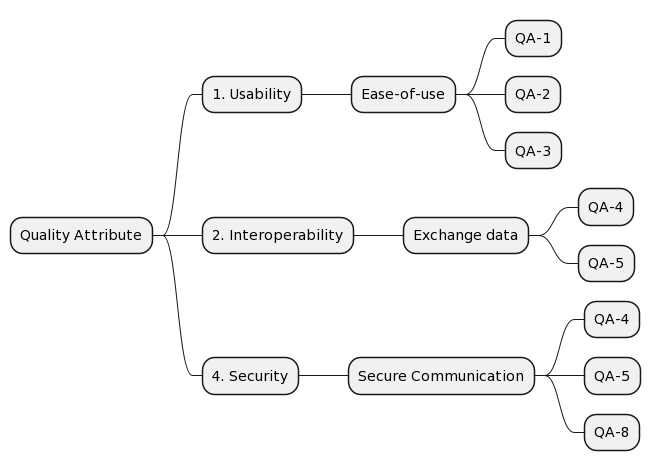
\includegraphics[width=0.7\textwidth]{assets/quality_tree.png}
    %\caption{Quality Tree}
    \label{fig:quality_tree}
\end{figure}

The next table presents the reason for the previous categorization regarding the priority of each quality attribute.

\begin{table}[H]
    \setstretch{1.0}
    \begin{tabularx}{\textwidth}{lXX}
        \toprule
        ID & Reasoning for \Glsplural{user} & Reasoning for Development Team  \\
        \midrule
        QA-1 & All important information should be there so his shop can be well promoted & 
        An initial registration with filter for the input is important, but aesthetically details are
        the goal now. \\
        QA-2 & Once he get something new, he wants to make it available & First we need to guarantee that no overrides occur
        than they see if it is promptly displayed. \\
        QA-3 & They want to browse and see all available options & Search engine can be very helpful, 
        but filtering can wait a litte, since it does not affect the app itself \\
        QA-4 & The most important is that they can use and purchase & This integration must be done fast and careful
        so no mistakes shows up. \\
        QA-5 & They just want to easily and secure pay, it does not matter how it works & The compliance with payment regulations is a must, since any mistake can costs huge fines
        and damage to the image of the company. \\
        QA-6 & They don't want to wast time with loading pages & The loading time can be fixed once there is a structure that allows
        loading in the first place.  \\
        QA-7 & They want to get confirmation that everything worked fine. & The communication between the \gls{API} and the payment provider show comply with all existing regulations. 
        Push notification can be added once the main feature works. \\
        QA-8 & That is something that they don't want to see, but want to make sure that it exists & Since the payment is processed by the third party operator, all concerns should be addressed to them
        and specified in the \glsfirst{SLA} \\
        \bottomrule
    \end{tabularx}
\end{table}


\subsection{Evaluation Scenarios} 
From the requirements, \ref{Requirement_Overview}, we could develop the following uses cases and depict the main quality 
attributes of this project. 

\begin{table}[H]
    \setstretch{1.0}
    \begin{tabularx}{\textwidth}{lX}
    \toprule
    Use Case & Description  \\
    \midrule
    UC-1: Register as \gls{client} & The \gls{client} registers an e-mail address.\\
    UC-2: Login & The \gls{client} logins in to the system. \\
    UC-3: Places an order & The \gls{client} chooses a \gls{provider}. \\
    UC-4: Register payment & The \gls{client} registers a payment method. \\
    UC-5: Register as \gls{provider} & The \gls{provider} registers their facility and products. \\
    UC-6: Update availability & The \gls{provider} uploads their product catalog. \\
    \bottomrule
    \end{tabularx}
    \label{table_use_case}
\end{table}

With the following use cases we will  be able to define the major quality attributes that are involved in the 
development of this application. They should be measurable and testable so we can verify if the system meets 
the needs our \glsplural{stakeholder} [\cite{refbook:DSHC}].

\begin{table}[H]
    \setstretch{1.0}
    \begin{tabularx}{\textwidth}{lcXc}
        \toprule
        ID & Quality Attribute & Scenario & Associated Use Case  \\
        \midrule
        QA-1 & Usability & A \gls{provider} is able to register his company, to specify the kind of products he offers 
        and upload a logo or picture of his shop and products in a easy and fast (within 5 Minutes) fashion. & UC-5 \\
        QA-2 & Usability & A \gls{provider} is able to update the offers at any time. &  UC-6 \\
        QA-3 & Usability & A \gls{client} is able to search and filter options. &  UC-6 \\
        QA-4 & Interoperability & A \gls{client} can register his e-mail using another account (Google, Microsoft, Facebook)
        in a \gls{federated login} & UC-1 \\
        QA-5 & Interoperability & A \gls{client} can pay the order using a \gls{mobile payment gateway} (e.g. Stripe, Square, PayPay, 
        SecurePay) & UC-4 \\
        %QA-5 & Performance & A \gls{client} registers his/her e-mail address and can immediately browse in the app. & UC-1 \\
        %QA-6 & Performance & A \gls{client} opens the app and he can immediately search for products or \glsplural{provider}. & UC-2 \\
        %QA-7 & Performance & A \gls{client} chooses a \gls{provider} and places his order. After the confirmation
        %of payment, a push-message is displayed in the app confirming the purchase. & UC-3 \\
        QA-8 & Security & The payment process should be secure and within the app. It should also give the \gls{client} the feeling
        of security. The \gls{client} inserts his payment information it is processed by the payment operator. & UC-4 \& QA-5 \\
        \bottomrule
    \end{tabularx}
\end{table}

\newpage
The defined quality attributes are represented in the following scenarios:

% add column id to the scenario

\begin{table}[H]
    \setstretch{1.0}
    \begin{tabularx}{\textwidth}{|c|X|X|X|}
        \hline
        \multicolumn{4}{c}{\textbf{Usability}} \\
        \hline
        \toprule
        \multicolumn{1}{|c|}{\textbf{Scenario}} & \multicolumn{3}{|c|}{\textbf{Value}} \\
        \midrule
        \multicolumn{1}{|c|}{ID} & \multicolumn{1}{|c|}{QS-1} & \multicolumn{1}{|c|}{QS-2} & \multicolumn{1}{|c|}{QS-3}  \\
        \hline
        Source & \Gls{provider} & Registered \Gls{provider} & \Gls{client}  \\
        \hline
        Stimulus & wants to register his shops & wants to make a last minute offer & wants to search/filter offers \\
        \hline
        Artifact & app & app & app \\
        \hline
        Environment & working time, during afternoon & peak period, between 4 and 7 pm on Friday & peak period, between 4 and 7 pm on Friday \\
        \hline
        Response & offer available in the app & immediate availability of the offer in the app & display of the filter/search output \\
        \hline
        Response Measure & How long did the registration and upload process take? How many and what kind of error messages did the \gls{provider} get?
        & How long did it take to upload an offer? How many and what kind of error messages did the \gls{provider} get? 
        & What kind of inputs did the user has to place until he finds what he wants? Did he have to type anything or were filter/search
        options available? How long it takes until the client finds a product? \\
        \bottomrule
    \end{tabularx}
\end{table}


% \begin{table}[H]
%     \begin{tabularx}{\textwidth}{|c|X|}
%         \hline
%         \multicolumn{2}{c}{\textbf{Usability - BACKUP}} \\
%         \hline
%         \toprule
%         \multicolumn{1}{c}{Scenario} & \multicolumn{1}{c}{Value} \\
%            \multicolumn{1}{|c|}{ID} & \multicolumn{1}{|c|}{QS-1} & \multicolumn{1}{|c|}{QS-2} & \multicolumn{1}{|c|}{QS-3}  \\
%            \hline
%         Source & \gls{provider} \\
%         Stimulus & wants to register his shops \\
%         Artifact & app \\
%         Environment & working time, during afternoon \\
%         Response & offer available in the app \\
%         Response Measure & How long did the registration and upload process take? How many and what kind of error messages
%         did the \gls{provider} get?\\
%          & \\
%         Source & Registered \gls{provider} \\
%         Stimulus & wants wants to make a last minute offer \\
%         Artifact & app \\
%         Environment & peak period, between 4 and 7 pm on Friday \\
%         Response & immediate availability of the offer in the app \\
%         Response Measure & How long did it take to upload an offer? How many and what kind of error messages did the 
%         \gls{provider} get? \\
%         & \\
%         Source & Registered \gls{client} \\
%         Stimulus & wants to search/filter offers \\
%         Artifact & app \\
%         Environment & peak period, between 4 and 7 pm on Friday \\
%         Response & display of the filter/search output \\
%         Response Measure & What kind of inputs did the user has to place until he finds what he wants?
%         Did he have to type anything or were filter/search options available? How long it takes until the client
%         finds a product? \\
%         \bottomrule
%     \end{tabularx}
% \end{table}

 \begin{table}[H]
    \setstretch{1.0}
    \begin{tabularx}{\textwidth}{|c|X|X|}
        \hline
        \multicolumn{3}{c}{\textbf{Interoperability}} \\
        \hline
        \toprule
        \multicolumn{1}{|c|}{\textbf{Scenario}} & \multicolumn{2}{|c|}{\textbf{Value}} \\
        \midrule
        \multicolumn{1}{|c|}{ID} & \multicolumn{1}{|c|}{QS-4} & \multicolumn{1}{|c|}{QS-5}  \\
        \hline
        Source & \Gls{client} & \Gls{client}  \\
        \hline
        Stimulus & wants register using a \gls{federated login} & wants to pay using existing mobile payment account \\
        \hline
        Artifact & app and \gls{federated login} provider & app and \gls{mobile payment gateway} \\
        \hline
        Environment & peak period (on the context of the \gls{federated login} provider) & peak period (on the context of the gateway) \\
        \hline
        Response & authentication succeed or failed & confirmation / declined \\
        \hline
        Response Measure & How much data was transmitted and how much was queued? Focus on System overload [\cite{refart:MKMS}]
        & Total amount generated data in the app that are transferred and processed and rejected by the gateway? Focus o connectivity 
        and system overload [\cite{refart:MKMS}] \\
        \bottomrule
    \end{tabularx}
\end{table}

% \begin{table}[H]
%     \begin{tabularx}{\textwidth}{|c|X|}
%         \hline
%         \multicolumn{2}{c}{\textbf{Interoperability - Backup}} \\
%         \hline
%         \toprule
%         \multicolumn{1}{c}{Scenario} & \multicolumn{1}{c}{Value} \\
%         \midrule
%         Source & \gls{client} \\
%         Stimulus & wants register using a \gls{federated login} \\
%         Artifact & app and \gls{federated login} provider  \\
%         Environment & peak period (on the context of the \gls{federated login} provider)\\
%         Response & authentication succeed or failed\\
%         Response Measure & How much data was transmitted and how much was queued? \\
%         Focus & System overload \cite{refart:MKMS} \\
%         & \\
%         Source & \gls{client} \\
%         Stimulus & wants to pay using existing mobile payment account \\
%         Artifact & app and \gls{mobile payment gateway}  \\
%         Environment & peak period (on the context of the gateway)\\
%         Response & confirmation / declined \\
%         Response Measure & Total amount generated data in the app that are transferred and processed and rejected
%         by the gateway \\
%         Focus & Connectivity and System overload \cite{refart:MKMS} \\
%         \bottomrule
%     \end{tabularx}
% \end{table}

% \begin{table}[H]
%     \setstretch{1.0}
%     \begin{tabularx}{\textwidth}{|c|X|X|X|}
%         \hline
%         \multicolumn{4}{c}{\textbf{Performance}} \\
%         \hline
%         \toprule
%         \multicolumn{1}{|c|}{\textbf{Scenario}} & \multicolumn{3}{|c|}{\textbf{Value}} \\
%         \midrule
%         \multicolumn{1}{|c|}{ID} & \multicolumn{1}{|c|}{QS-6} & \multicolumn{1}{|c|}{QS-7} \\
%         \hline
%         Source & \Gls{client} & \Gls{client} & \Gls{client}  \\
%         \hline
%         Stimulus & wishes to create an account & wants to search for a \gls{provider} & places an order \\
%         \hline
%         Artifact & app & app & app \\
%         \hline
%         Environment & weekend between 3 and 7 PM & peak period, between 6 and 7 pm on a Friday & peak period, between 6 and 7 pm on a Friday \\
%         \hline
%         Response & immediate access to the app  & immediate access to the offers  & confirmation of payment / payment declined \\
%         \hline
%         Response Measure & time between confirmation and access & how quickly does the client's device get update of availabilities 
%         & How long did take until the client get the confirmation/declined of payment? \\
%         \bottomrule
%     \end{tabularx}
% \end{table}


% \begin{table}[H]
%     \begin{tabularx}{\textwidth}{|c|X|}
%         \hline
%         \multicolumn{2}{c}{\textbf{Performance - Backup}} \\
%         \hline
%         \toprule
%         \multicolumn{1}{c}{Scenario} & \multicolumn{1}{c}{Value} \\
%         \midrule
%         Source & \gls{client}  \\
%         Stimulus & wishes to create an account \\
%         Artifact & app \\
%         Environment & weekend between 3 and 7 PM \\
%         Response & immediate access to the app \\
%         Response Measure & time between confirmation and access \\
%          & \\
%         Source & \gls{client}  \\
%         Stimulus & wants to search for a \gls{provider} \\
%         Artifact & app \\
%         Environment & peak period, between 6 and 7 pm on a Friday \\
%         Response & immediate access to the offers \\
%         Response Measure & how quickly does the client's device get update of availabilities \\
%         & \\
%         Source & \gls{client}  \\
%         Stimulus & places an order \\
%         Artifact & platform \\
%         Environment & peak period, between 6 and 7 pm on a Friday \\
%         Response & confirmation of payment / payment declined \\
%         Response Measure & How long did take until the client get the confirmation/declined of payment?\\
%         \bottomrule
%     \end{tabularx}
% \end{table}

\begin{table}[H]
    \setstretch{1.0}
    \begin{tabularx}{\textwidth}{|c|X|X|}
        \hline
        \multicolumn{3}{c}{\textbf{Security}} \\
        \hline
        \toprule
        \multicolumn{1}{|c|}{\textbf{Scenario}} & \multicolumn{2}{|c|}{\textbf{Value}} \\
        \midrule
        \multicolumn{1}{|c|}{ID} & \multicolumn{1}{|c|}{QS-6} & \multicolumn{1}{|c|}{QS-7}  \\
        \hline
        Source & \Gls{client} & \Gls{client} \\
        \hline
        Stimulus & clicks on registration using an existing login & click on pay using an existing mobile payment account \\
        \hline
        Artifact & app, \gls{API Gateway} and \gls{federated login} provider & app, \gls{microservice} and \gls{mobile payment gateway} \\
        \hline
        Environment & peak period (on the context of the \gls{federated login} provider) & peak period (on the context of the gateway) \\
        \hline
        Response & authentication succeed or failed & confirmation / declined \\
        \hline
        Response Measure & Required time and effort to intercept and/or block requests (create \glsfirst{DoS})
        & Extension and impact to image/damage of the app/company in case of attack \\
        \bottomrule
    \end{tabularx}
\end{table}